\textbf{Una lista que muestre la región, el estado y el total de clientes que se tienen, considerando que los clientes deben
haber realizado órdenes con al menos 6 productos durante 2014 o 2015. Ordenar la información por región y estado..} \vspace{.3cm}

Primero el Álgebra Relacional es:

\begin{center}
    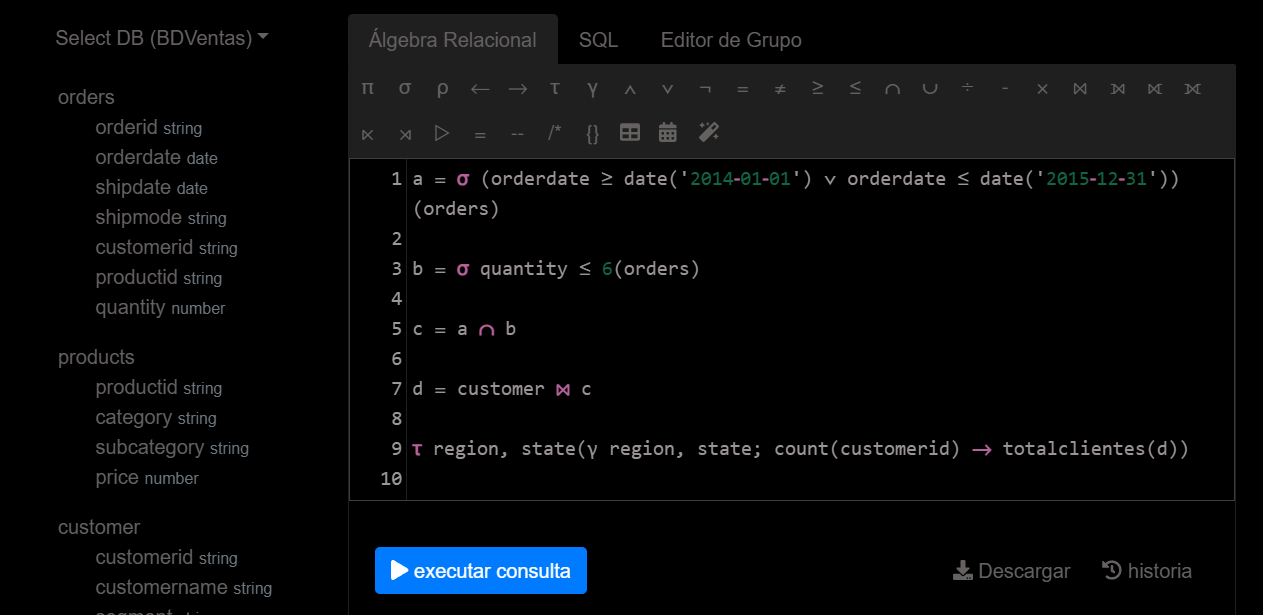
\includegraphics[width=14cm]{resources/pregunta2/2.6.1.png}
\end{center}


El resultado de las tablas es:

\begin{center}
    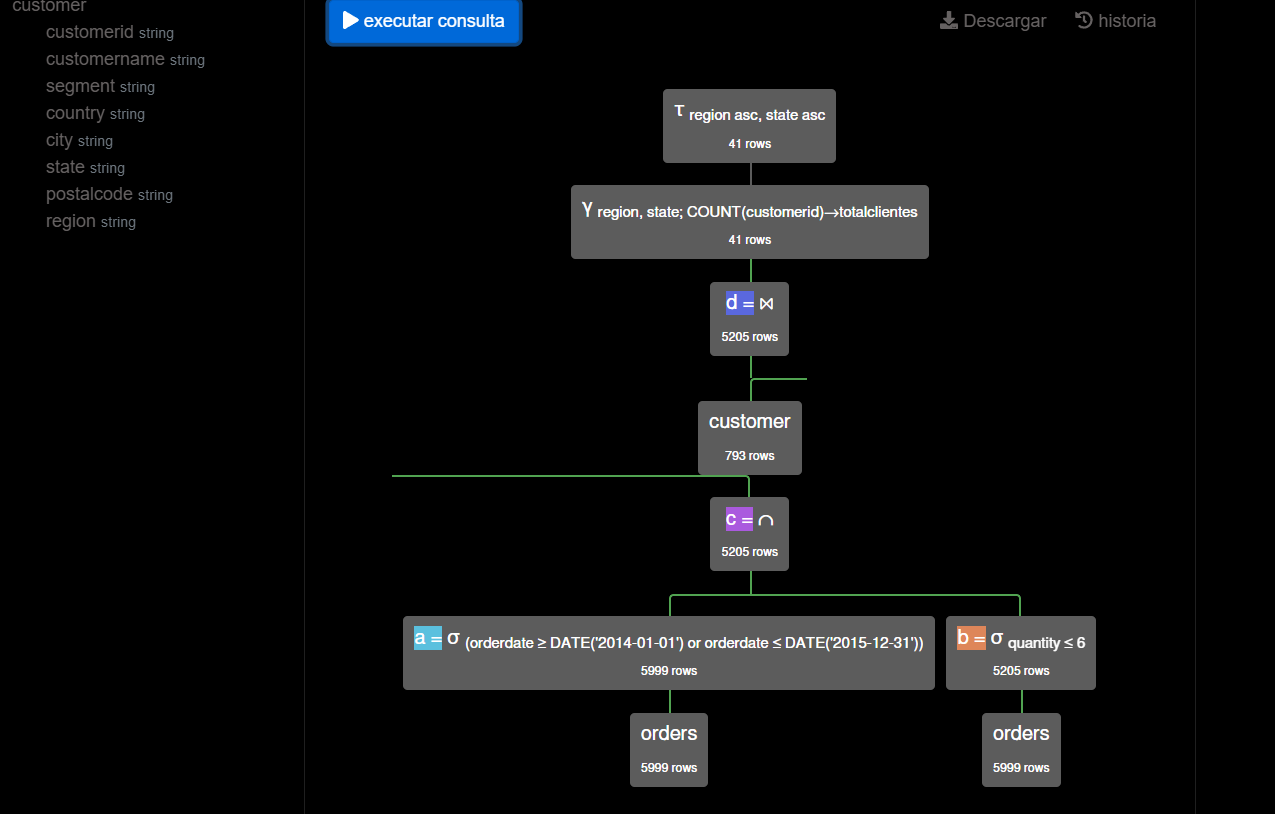
\includegraphics[width=14cm]{resources/pregunta2/2.6.2.png}
\end{center}


\begin{center}
    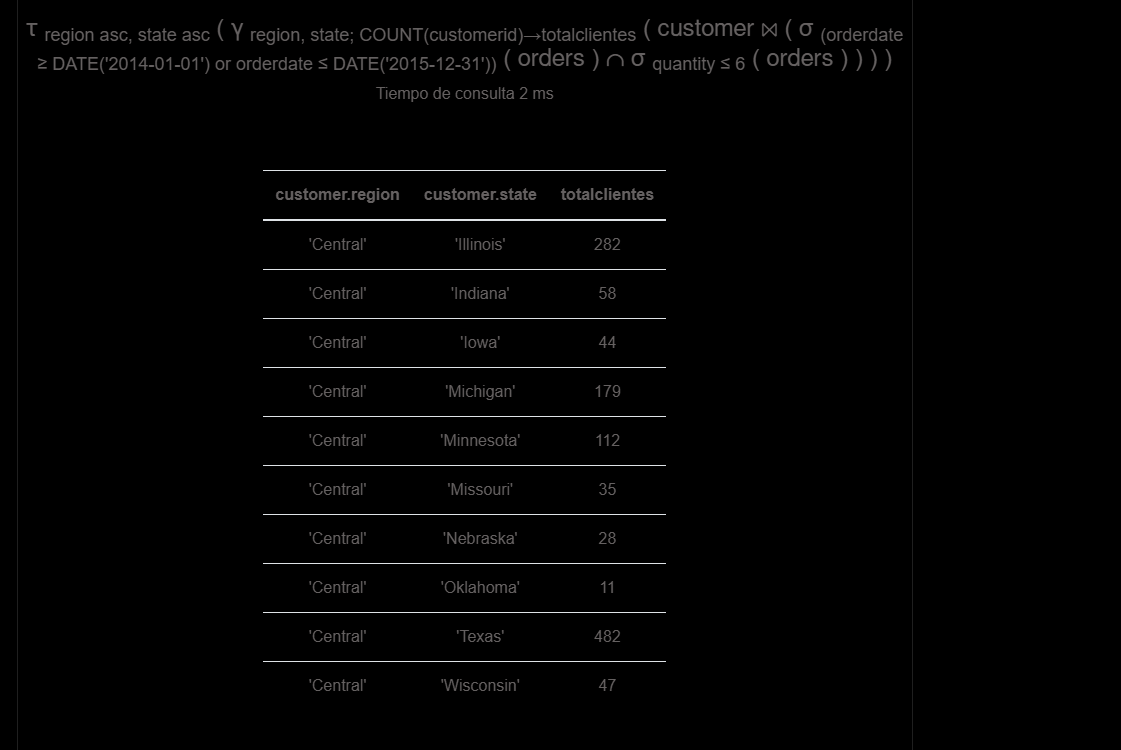
\includegraphics[width=14cm]{resources/pregunta2/2.6.3.png}
\end{center}
